\chapter{Design}
In this chapter we will discuss the architecture of the prototype.
It's divided into two section: Dataset and Model. Since
the dataset is standalone component, this seems to be
a reasonable separation. To make it clear, dataset would be a component
which holds the training, validation and test data including all relevant
functionality that can or should be performed on the
data(this is explained more detailed in \autoref{sec:design_data}).
Model would be a component, which accepts the data(dataset component), performs
training on the training data, and then makes inference on the test dataset.
In other words, model would be everything what is related to building,
training and evaluation of neural networks and reinforcement learning environment.



\section{Dataset}
\label{sec:design_data}

Dataset is component which is responsible for data holding. It should
accept original MNIST dataset and transform it into dataset described
in \autoref{sec:analysis_dataset}.

\paragraph{MNIST Dataset} is dataset of scanned handwritten images, each labeled
from 0 to 9. You can see an example of 4 digits in figure \ref{fig:mnist}.
Additionally, it includes label for each of the image.

\begin{figure}[h!]
	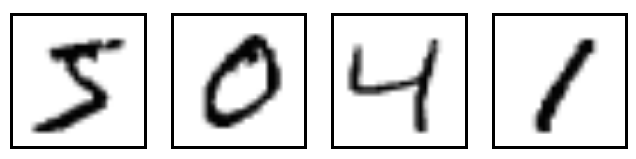
\includegraphics[width=\linewidth,scale=0.4]{MNIST}
	\caption{MNIST example}
	\label{fig:mnist}
\end{figure}

For example, in the figure \ref{fig:mnist} the labels are 5, 0, 4 and 1.
Each images consist of $28\times28$ pixels, therefore an MNIST image would
be an array of size $784$. To each of the image, a label is assigned,
which provides the ground truth.

\subparagraph{MNIST from TensorFlow}

TensorFlow provides a small class \lstinline{Dataset}\footnote{
The class is implemented here: https://github.com/tensorflow/tensorflow/blob/master/tensorflow/contrib/learn/python/learn/datasets/mnist.py
} which stores MNIST data and splits it into training,
validation and test data. TensorFlow also provides functions for iterating
over the batches as well as the function which downloads and read
the original data
from MNIST web site. Taking this into account, in this work we will abstract from
downloading and reading MNIST data by using this class. We'll refer
to this class as \emph{MNIST tf-dataset class}

% Remove this:
% \begin{lstlisting}[language=Python]
% from tensorflow.examples.tutorials.mnist import input_data
% mnist = input_data.read_data_sets("MNIST_data/", one_hot=True)
% \end{lstlisting}
This two lines will download the data and store into "MNIST_data/" directory.

It is common knowledge that google take a special care about the quality of their code,
therefore our dataset component should have the similar
behaviour and functionality as MNIST tf-dataset class. Another reason for that
is that we want to stay consistent with tensorFlow practices as we use this library
in this work.

% Dataset is a non-real world data, but may behave and represent similar
% task as it could in real world data.
% \paragraph{explain original MNIST data, what is there, how does this work,
% and tf class is used to provide the utility}

% \paragraph{Obstacles} Using the procedure described in \autoref{sec:design_data}
% to create the dataset several obstacles can arise.
% we need to make sure that no same non-noise picture come up with in the dataset.

% To make the dataset
% By build the dataset, we need to consider following

% we want the model to generalise on unseen data.

\subsection{Class overview}

Before proceeding with the classes overview, it can be helpful
to make a concrete example of how the dataset described in
\autoref{sec:analysis_dataset} can look like.

\paragraph{Example} In this example we will describe dataset with two classes
Let's first choose the parameters $n$ and $k$,
which represents amount of images in a group and amount of noise images
in a group respectively. While $k$
should be different for both classes, $n$ remains the same.
Let $n$ be equal to $5$, $k$ for the first class be and $3$: $k_1 = 3$
for the second class be $4$: $k_2 = 4$. Let's choose the digit for the non-noise
data: $\{1\}$. Consequentially the noise-image will
be: $\{0, 2, 3, 4, 5, 6, 7, 8, 9\}$.
So one sample of the above mentioned setup can look like this:

\begin{lstlisting}[language=Python][h!]
	[noise_image, non_noise_image, noise_image, non_noise_image, noise_image ] # class 1
	[non_noise_image, noise_image, noise_image, noise_image, noise_image ] # class 2
\end{lstlisting}

Or with numbers:
\begin{lstlisting}[language=Python][h!]
	[9, 1, 8, 1, 7 ] # class 1
	[1, 3, 6, 4, 3 ] # class 2
\end{lstlisting}

Hopefully, it gives you a sense how the data should appear.

\paragraph{Classes}

After careful analysis, it was decided that in order to implement
the desired dataset, three classes are required:
\begin{itemize}
	\item IndexGenerator - the purpose of this class is to generate indexes for
		noise images. Imagine situation, where all of noise data is placed into
		the same indexes. Will the model learn this indexes and look only at
		them? Or will model ignore this stability? Because this question seems
		to be heuristic, this class will control the indexes where noise image
		will be located at.
	\item DummyDataset - The purpose of this class is to hold MNIST images
		and labels. Additionally, this class provides some auxiliary functionality
		like permutation of the data.
	\item GroupDataset - this is our desired dataset. It should be flexible
		enough to generate and hold the data for all classes. In terms of
		available methods, this class behaves the same way as NIST tf-dataset class
		once initialized.
\end{itemize}

Dataset component should be flexible enough in order to be similar to real problems,
to be able to experiment with different amount of classes, and
different variations of noises classes. Since we have only limited amount of MNIST data,
we need to also make sure that this data is properly used. GroupDataset takes
care of it by carefully choosing the data from original MNIST dataset and putting
them into the group to avoid if possible two same samples in the dataset by building
combinations of noise-data and non-noise data.

\subsection{UML class diagram}

In the figure \ref{fig:dataset_uml} you can see UML diagram of the dataset package
as well as the it's connection to tf-dataset class. As you can see from the UML
class diagram.
\lstinline{GroupDataset} class holds two \lstinline{DummyDataset}, one for
non-noise data and one for noise-data. This is exactly the way
we described it in \autoref{sec:design_data}.
\begin{figure}
	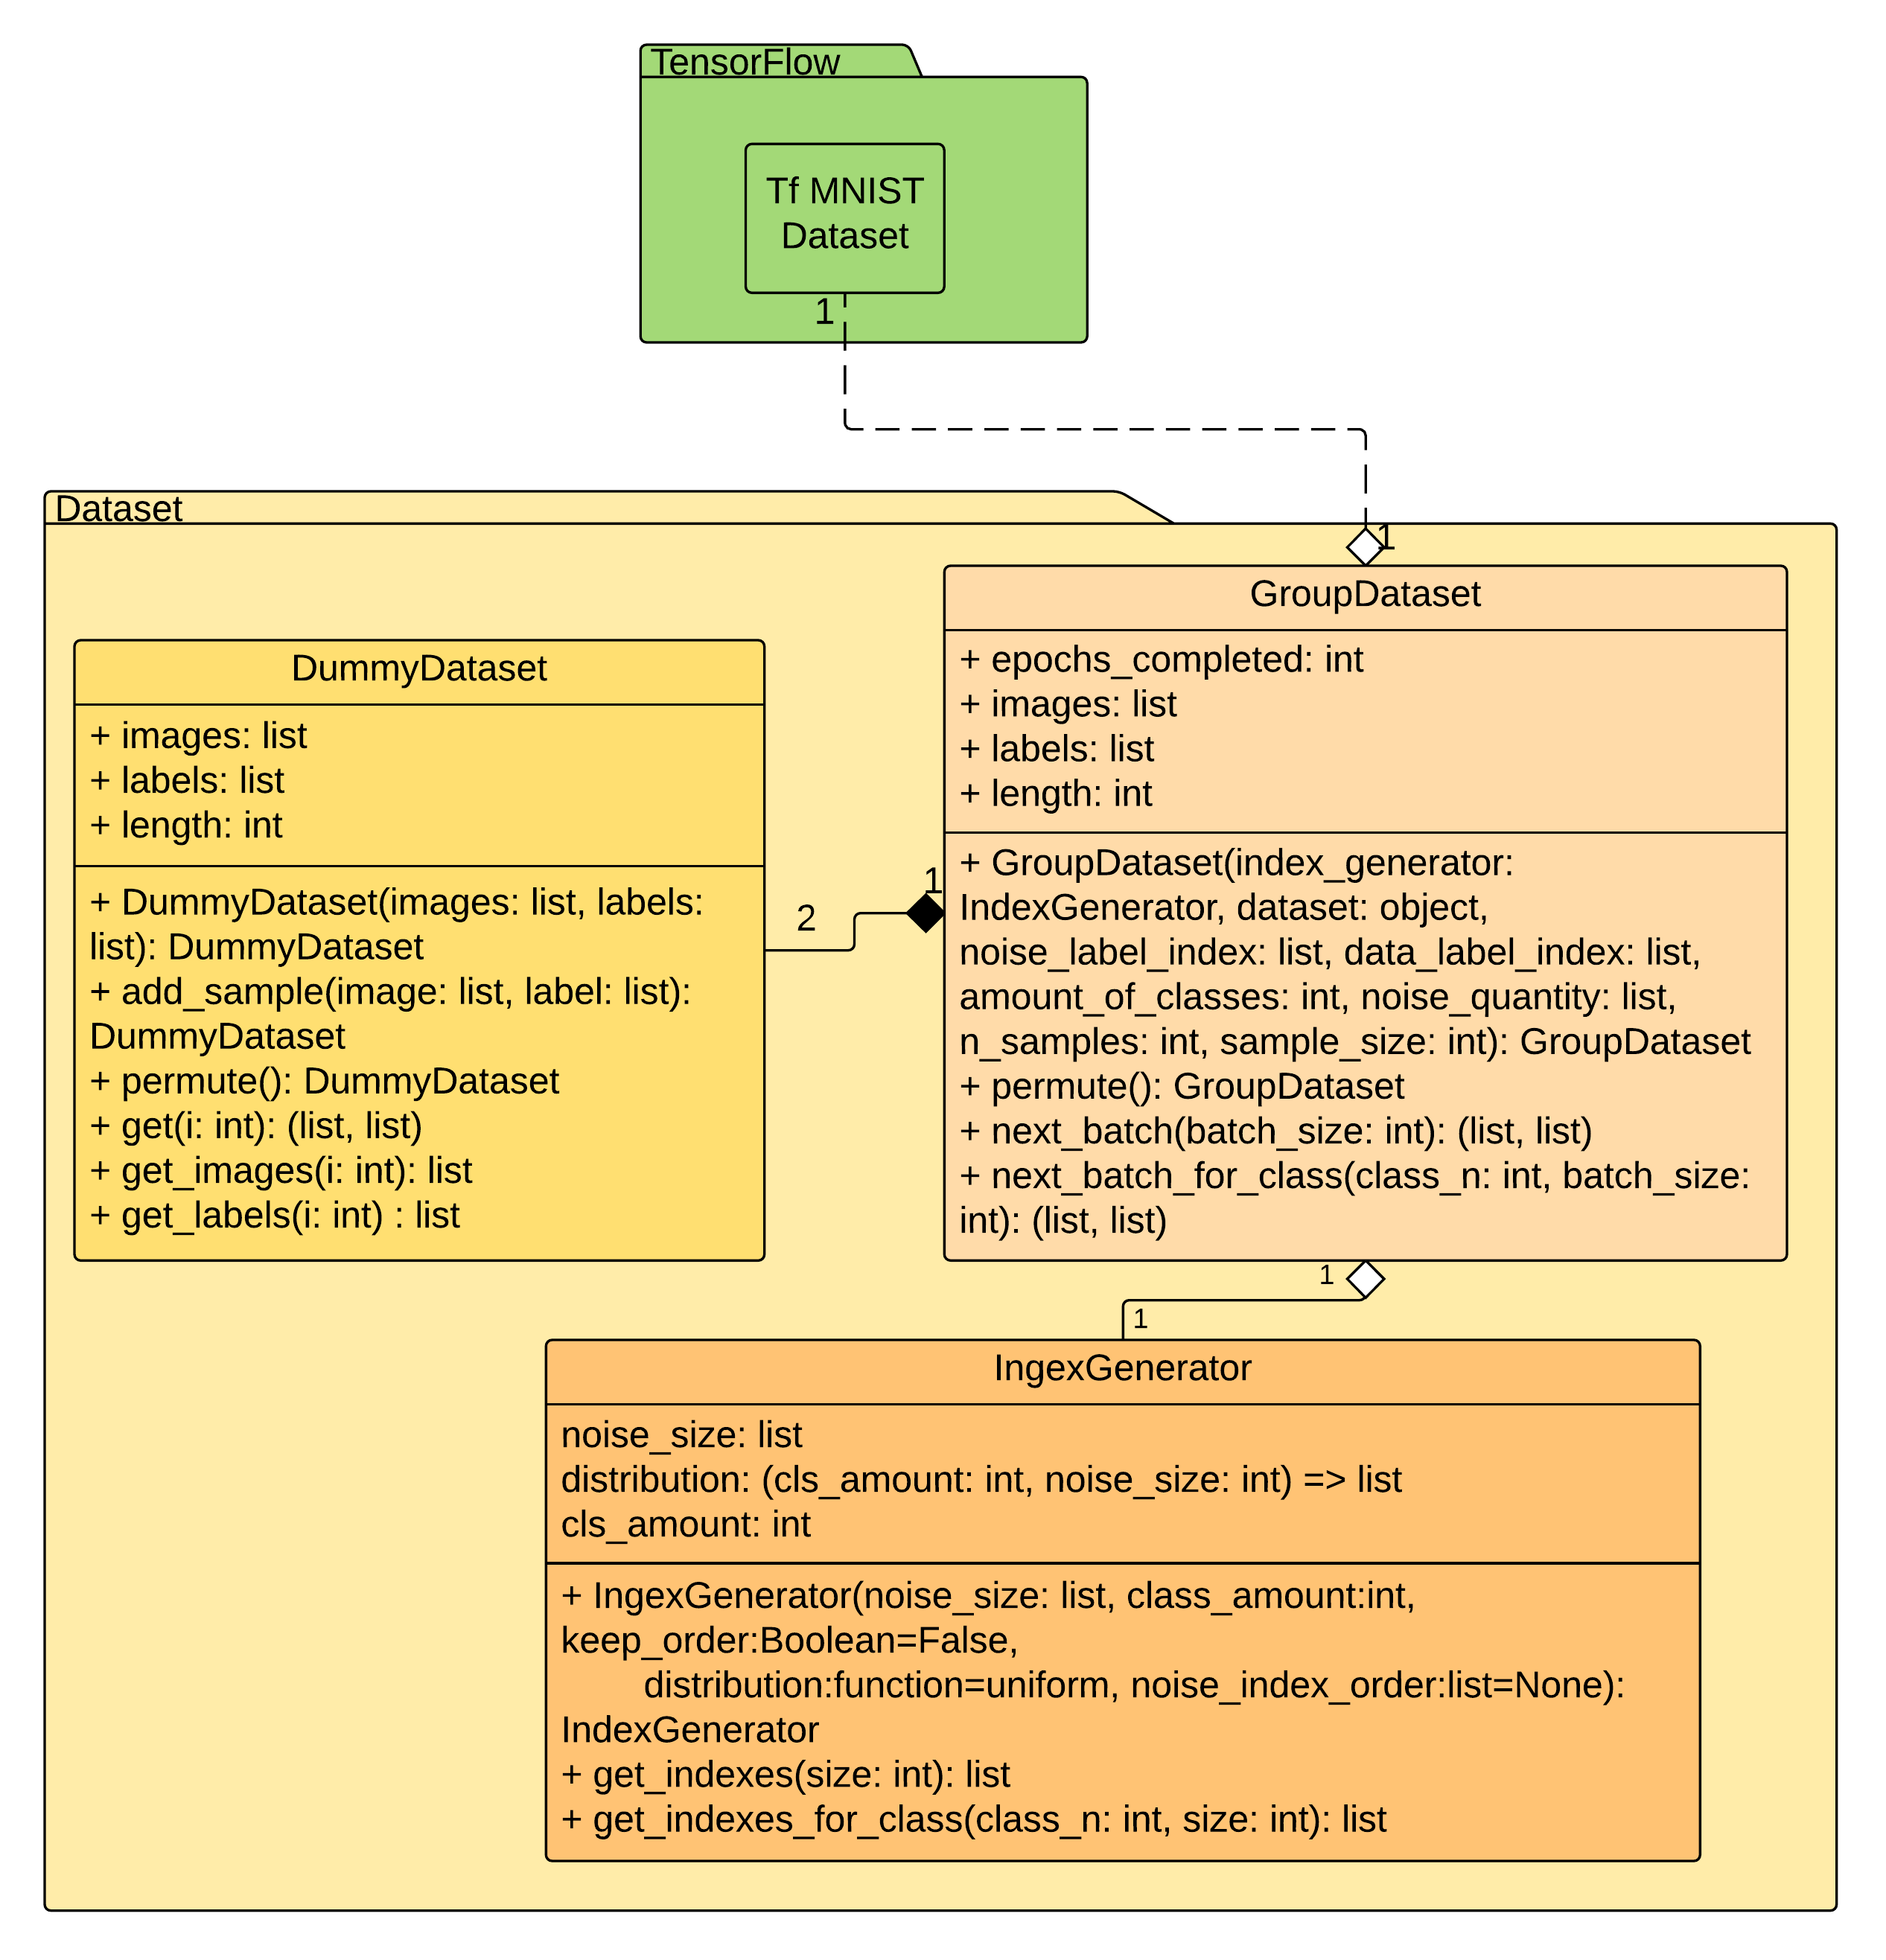
\includegraphics[width=\linewidth]{Dataset_UML}
	\caption{UML class diagram of the dataset module}
	\label{fig:dataset_uml}
\end{figure}

\paragraph{Code pattern} As we can see from the UML class in the figure
\ref{fig:dataset_uml}, we have three classes. It would be also possible
merge the classes, however, this contradicts "Single Responsibility Principle"
that one class should only have one responsibility \cite{martin2003agile}.
Therefore, dividing this into two classes allows us to clearly
define responsibilities. Consequently, this separations seems to be reasonable.

As you might notice from UML class diagram, some of the function like
\lstinline{add_sample} in \lstinline{DummyDataset} returns the object itself: \lstinline{DummyDataset}.
This is an example of Cascade code pattern described in \autoref{sec:quality_concerns}.
% As you might notice from UML class diagram, that \lstinline{GroupDataset} can inherit
% \lstinline{DummyDataset} as they have similar properties,
% but as "Composition over Inhertitance" states, it
% not always a good idea.

%
% inderect variable access. (e.g.)

% TODO:
% look over the Dataset implementation,
% write all documentation
% draw uml diagrams
%
%
%
%
%

% \paragraph{Requirements} Like why do we need index generator
% including flexibility
% \paragraph{Inspiration fromt the tf class dataset}
%
% inpsiration from dataset class from tensor flow: link
% https://github.com/tensorflow/tensorflow/blob/master/tensorflow/contrib/learn/python/learn/datasets/mnist.py
% that should perform similar action to
% The function requirement to the dataset can be formulated as

% \paragraph{
% 	not learning any dependency,
% 	explain that we want to avoid the same samples in a group to avoid that
% }
% model will learn dependency and etc.

% \paragraph{
% 	explain shortly about combinations of MNIST data, how to achieve the best data
% }
%
% \paragraph{then show the uml diagram of dataset}
% including: Class overview
%
% \paragraph{explain what is purpose of each of the class. }


\section{Model}
\label{sec:design_model}

% \paragraph{Why did you choose picker network?}
We described three approaches of how to extend the RAM model
in \autoref{sec:extension}. The implementation of this work
will only concentrate on method described as picker network.
This is because of the simplicity of this approach.

%TODO: patterns https://www.toptal.com/python/python-design-patterns

\paragraph{about why OO programming is not ALMOST suited and why it should be more functional}


\paragraph{The architecture as a whole}
\paragraph{Possible classes, overview}
\paragraph{UML diagram}
\paragraph{back up the classes with design patterns}

\paragraph{the flow of the data via function}


\subsection{Configuration of the project, what can be configured, the complexity of the model}





the curent desing is using the approach
described in \autoref{ssec:picker_net}.

Basically explain the flow of input data, all losses, and baselines, and etc.
if there is anything relative to the structure in the code use the references to the design patters
Show all classes, write the documentation for those, or at least briefly explain the purpose.
The process of training, maybe explain the whole idea behind this
	seperation of dataset into validation, test, training.
look at the other bachelorarbeits and look of what they wrote there
think about whether it's possible to combine the design and implemntation chapters



* Entwurfsstrategie, Beschreibungen funktionaler und nich
 funktionaler Anforderungen, Einsatz von Mustern und
 Bibliotheken, Softwarearchitektur, Verwendung von Datentypen und
 Datenstrukturen, Algorithmen, Mensch-Maschine-Schnittstelle;
